%1. Intro White-box, overview of analysis
%2. Explaining some analyzing strats that are out there
%3. VaRA, explain what vara does roughly (Regions)
%4. Vara TS Experiment explain
%5  TEF Report and how we evaluate them
%6. Using data to build multiple perf-influcence models


\colorlet{punct}{red!60!black}
\definecolor{background}{HTML}{EEEEEE}
\definecolor{delim}{RGB}{20,105,176}
\colorlet{numb}{magenta!60!black}
\lstdefinelanguage{json}{
    basicstyle=\normalfont\ttfamily,
    numbers=left,
    numberstyle=\scriptsize,
    stepnumber=1,
    numbersep=8pt,
    showstringspaces=false,
    breaklines=true,
    frame=lines,
    backgroundcolor=\color{background},
    literate=
     *{0}{{{\color{numb}0}}}{1}
      {1}{{{\color{numb}1}}}{1}
      {2}{{{\color{numb}2}}}{1}
      {3}{{{\color{numb}3}}}{1}
      {4}{{{\color{numb}4}}}{1}
      {5}{{{\color{numb}5}}}{1}
      {6}{{{\color{numb}6}}}{1}
      {7}{{{\color{numb}7}}}{1}
      {8}{{{\color{numb}8}}}{1}
      {9}{{{\color{numb}9}}}{1}
      {:}{{{\color{punct}{:}}}}{1}
      {,}{{{\color{punct}{,}}}}{1}
      {\{}{{{\color{delim}{\{}}}}{1}
      {\}}{{{\color{delim}{\}}}}}{1}
      {[}{{{\color{delim}{[}}}}{1}
      {]}{{{\color{delim}{]}}}}{1},
}


%************************************************
\section{White-box Model}\label{ch:Whitebox}
%************************************************

A black-box analysis is very useful for systems where we do not have access to the source code, but if we do, it
would be a waste not to work with this additional information. 
This enables a white-box analysis 
that uses this new information to derive a \perfInfluenceModel, which is built differently than the black-box approach.


\begin{figure}[h]
    \centering
    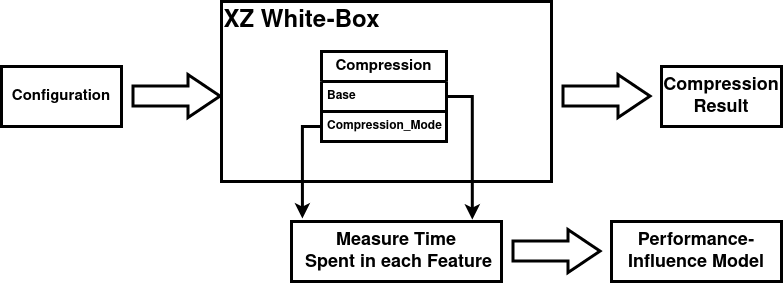
\includegraphics[scale=0.6]{gfx/whitebox_2.png}
    \caption{A white-box analysis of XZ}
    \label{fig:WBxz}
\end{figure}

We now analyze the example system from \autoref{fig:xz} using a white-box analysis. In \autoref{fig:WBxz} we can now see the inner workings of 
XZ when we are compressing a file. During compression, we can measure the time spent by XZ in the different features, in our example we measure 
the time spent in $Base$ and $Compression\_Mode$, after the system finished the process we have collected all the measurements which we 
then use to build a \perfInfluenceModel for this configuration.

This section explains current state of the art strategies and the strategies they use to collect the measurements of each feature in
\autoref{analyzing-strats}. We then explain the analyzing tool we use, a variability aware region analyzer and its underlying principles
in \autoref{VaRA}. Then, in \autoref{trace-event} we explain how to build the \perfInfluenceModel using the data we collected.



%\subsection{Disadvantages of White-Box}
%When using white-box model we clearly see how a feature interacts with another feature, due to that we do not need to sample our configuration space like
%we do in the black-box, meaning we do not face the problem of combinatorial explosion. 
%Neither do we have to handle multicollinearity features differently, since we can see in what extend they influence each other. 
%The example from \ref{ColinearF} would be no problem for the white-box model since we are aware that $c$ and $d$ do not interact with one another and can
%therefore assign them the precise amount of time they spend in their code region respectively, whereas the black-box model needs to infer this information.

%With the surplus of information, the white-box model faces different challenges. 
%First and foremost, to analyze larger systems we need a robust strategy and in depth code comprehension.

\subsection{Analyzing Strategies}\label{analyzing-strats}
The analysis of programs is in itself a highly complex subject, and it is not a trivial task to use one program to perform an analysis on another system.
In our case, we first need to find out which parts of the code corresponds to which feature.

To address this problem, several solutions have been proposed, Weber et. al. \cite{White-box-Profiling} uses a profiling approach to generate 
performance-influence models that depict configurability on a method level. To achieve this, they first used JProflier a coarse-grained profiler,
to learn a performance influence model for every method that have been learned successfully. 
To identify the hard to learn methods they use a filtering techniques and then KIEKER, a fine-grained profiler, to learn these methods.

Velez et. al. introduced us to ConfigCrusher \cite{ConfigCrusher} a white-box analysis, that uses a static data-flow analysis to see how features influence 
variables and the control-flow of the system. In addition, ConfigCrusher leverages three insights about configurable systems from previous works, namely
irrelevance, orthogonality and low interaction degree. Irrelevance is used to identify features that are relevant to the systems data-flow, thereby
reducing the number of configurations required to analyze the system. Orthogonality is used to identify features that do not interact with each other and
therefore can be measured together. Since only a few features interact with each other, ConfigCrusher focuses on the configurations with interacting 
features to reduce the number of configurations to be analyzed. 
From these findings, two techniques are developed, namely compression and composition.
Compression is used to reduce the number of configurations required to analyze the system
by simultaneously analyzing regions that are independent of each other so that they can use a single configuration to 
analyze different features. 
Whereas composition takes advantage of the fact that \perfInfluenceModel can be build compositionally, by building a performance-influcence model for each 
region separately and then assembling all local \perfInfluenceModel into one model for the entire system.

Siegmund et. al. introduced us to Comprex \cite{Comprex}, which built on the works of ConfigCrusher but uses dynamic taint analysis instead of static
analysis to determine how and to what extent features affect the control flow of the given system.

Both Comprex and ConfigCrusher use the techniques of compression and composition. The main difference between the two analysis methods is Comprex 
uses a dyanmic taint analysis while ConfigCrusher uses a static data-flow analysis, both are used to depict configurability on a feature level, 
while Weber et. al. depicts configurability on a method level. 

After we have figured out which parts of the code correspond to which function, we still instrument the code to measure the time spent on each feature.

\subsection{VaRA}\label{VaRA}
To analyze the system we are interested in, we use VaRA, a variability aware region analyzer, a framework for analyzing software built on LLVM
and the VaRA Tool Suite\footnote{Visited at 14.03.2022 \url{https://vara.readthedocs.io}}, developed at Saarland University. 
The purpose of VaRA is to provide various analyses for systems where the user only needs to focus on the high-level conceptual information of the 
system, while VaRA handles the low-level-details. 
Since VaRA is built on top of LLVM, it is able to analyze systems written in languages that can be compiled by LLVM, such as C, C++ or Rust. 

VaRA is able to perform a static analysis to analyze the source code directly. The way VaRA does that is by analyzing the
abstract syntax tree of the system and locate the if-blocks along with variables that represent features together they form 
feature regions. Then, VaRA instruments the binary so that we are able to track the time spent in each feature region
during the dynamic analysis when we run the binary. \cite{VaRA-Flo}

\begin{algorithm}
    \caption{Feature region}\label{alg:Vara_feature_regios}
    \begin{algorithmic}[1]            
        \State $\textit{Encryption} \gets \textit{True or False}$\label{alg:feature_variable}
        \If{$Encryption$} 
            \State $\textit{...}$
        \Else
            \State $\textit{...}$
        \EndIf    
    \end{algorithmic}
\end{algorithm}

In \hyperref[alg:Vara_feature_regios]{Algorithm \ref*{alg:Vara_feature_regios}} we can see the structure of the $Encryption$ feature region. The
feature variable in \hyperref[alg:feature_variable]{line \ref{alg:feature_variable}} represents whether $Encryption$ is selected or deselected, 
depending on $Encryption$ either the $then$ or $else$ branch is executed. 
Together, these two branches form an $Encryption$ feature region.

However, VaRA is not able to automatically detect which variables represent features. Therefore, we provide VaRA with a feature
model that contains the features of the system together with their location within the code. 
For \hyperref[alg:Vara_feature_regios]{Algorithm \ref*{alg:Vara_feature_regios}}, we would note that the feature variable
$Encryption$ is in \hyperref[alg:feature_variable]{line \ref{alg:feature_variable}}.

After identifying all the feature regions of each feature, we run the instrumented binary to analyze the time 
spent in each feature region \cite{VaRA-Flo}.


\subsubsection{VaRA Tool Suite}
We use VaRA in combination with the VaRA Tool-Suite, which allows us to use VaRA by specifying an experiment to analyze a particular project. 

An experiment inside the VaRA Tool-Suite is a concept which specify how we want to analyze a software project, this allows us to make the analysis
easy to reproduce and repeat.
The project specifies the system we want to analyze. Here we define how we build the system or which version of the system we want to study. 

In our example of \autoref{fig:WBxz}, the project would be XZ and would specify which version of XZ we want to analyze and how the binary is build.
The experiment defines which configuration we want to analyze and how we want to analyze it, in our case we want to analyze 
XZ with VaRA, we also specify the report we want our measurements stored in, like the trace event format in \ref{trace-event}.

\subsection{Trace Event Format}\label{trace-event}
When we analyze a system, it is very rare that we enter the region of a feature only once and afterwards stop interacting with regions of that feature. 
Most often, a feature affect multiple regions, and we visit not just one region but many during different phases of the program execution,
each time measuring the time spent in each region.
We collect all these measurements
in a trace event format (TEF) \footnote{Visited at 15.03.2022 \url{https://docs.google.com/document/d/1CvAClvFfyA5R-PhYUmn5OOQtYMH4h6I0nSsKchNAySU}} report.

Every time we enter or leave a region that is affected by a feature, a trace event is triggered that contains the following information:

\begin{lstlisting}[caption={Trace event},captionpos=b,language=json,firstnumber=1,label={event}]
"name": "Base",
"cat": "Feature",
"ph": "B",
"ts": 0,
"pid": 726119,
"tid": 726119,
"args": {
    "ID": 0
}\end{lstlisting}
    
In \autoref{event} we see how a trace event is structured. Each trace event contains a $name$ that refers to the names of the features that affect this
region, $ph$ represents the event type, while $B$ signals the beginning and $E$ the end of an event.
All events contain a timestamp $ts$ that refers to the time in milliseconds when the event began or ended.
$Args$ contain an $ID$ that refers to each event, so the event that initiates the beginning $E$ of a region has the same $ID$ as the event that signals when
we leave the region with $E$.

After the system finished its execution we have to transform the TEF report into a \perfInfluenceModel by aggregating all events. To do so we sum up 
all the time spent in each region and attribute this time to the feature that influenced that region. % Maybe more detail 
Therefore, the \perfInfluenceModel is build by adding a term for each feature and feature interaction we measured.  